\section{Introduction}\label{sec:introduction}


Pensions account for a large share of public sector expenditures in developed and developing countries. In 2020, the average spending on pensions among OECD countries was roughly 8\% of GDP, while in emerging markets and middle income economies, it was close to 4\% of GDP.\footnote{There is significant heterogeneity in spending, even among rich OECD countries. Spending is a bit more than 3\% of GDP in Ireland and Chile, and more than 17\% in Italy and Greece. See \textcite{OECDpen}.} Given their size, it is no surprise that the design of social security systems remains a central concern in policy debates. As populations age, policymakers must navigate difficult trade-offs among intergenerational equity, fiscal sustainability, and labor market efficiency. Moreover, pension arrangements are not determined by actuarial considerations alone: they are the outcome of political processes in which heterogeneous voters and organized interests shape the level and composition of benefits and contributions. A political-economy perspective is therefore critical for understanding why countries differ in social security tax rates, replacement rates, and coverage, and for assessing the likely effects of proposed reforms. Understanding this politico-economic equilibrium is therefore essential to explain observed cross-country variation in social security tax rates, replacement rates, and coverage, as well as to evaluate ongoing reforms.

Pension systems vary widely along two key dimensions. The first concerns eligibility and coverage: while some systems condition benefits on contributory histories, others offer universal entitlements. The second concerns the link between earnings and benefits: Bismarckian systems tie pensions closely to past income, whereas Beveridgean systems provide flat-rate benefits. Both dimensions critically shape the labor supply incentives of workers, the redistribution embedded in the system, and the coalition of voters supporting it. Yet, despite the empirical relevance of these design features, few politico-economic models have systematically integrated them.\footnote{A notable exception is Conde-Ruiz and Profeta (2007), who study redistributional aspects of pensions, but without embedding the political game in an intertemporal equilibrium with capital accumulation.} We seek to address this gap in the literature with a dynamic politico-economic model to study how pension design affects equilibrium tax rates, savings and labor supply.

To analyze the effects of pension system characteristics, we use a tractable overlapping generations model with capital formation and heterogeneous agents. In the model, households make decisions about consumption, savings, and labor supply, and as voters, they choose among policies on labor income taxes and retirement benefits. Policy preferences vary by income and age; we model the resolution of these conflicts through probabilistic voting with elections taking place every period. Policy decisions not only impact economic outcomes, but also affect future policy decisions. Voters take these indirect effects into account. We focus on Markov perfect equilibria and assume that only fundamental state variables enter the equilibrium relationship between state variables and future policy choices. 

A share of young households are employed in a formal labor market and make a consumption saving decision as well as a labor supply decision. These formal households differ in their labor productivity. The remaining share of young households work in an informal sector or get income from home production. We denote them informal or displaced households, and we allow them to save through informal mechanisms, i.e.\ their savings do not contribute to capital accumulation.\footnote{To derive some analytical results we make the simplifying assumption that informal households are hand-to-mouth receiving an endowment of goods when old.} 
Labor supplied in the formal market is more productive but taxed; home production is not taxed. We adopt \textcite{GreenwoodHH88a1} preferences, which allow for a tractable characterization of labor supply. In a static setting, labor supply depends solely on the after-tax wage. In our dynamic framework, however, it is also shaped by workers’ expectations about how their current effort influences future pension benefits. 

Introducing informal households into the model allows us to address two challenges to social security systems across the world. First, in developing countries informal households constitute a large share of the population and would fail to qualify for pensions under strict contributive systems. Second, in developed countries they capture the evolution of emerging work structures characterized by low job security, including platform work, zero-hour contracts, and various forms of self-employment. Despite currently constituting a minor fraction of overall employment, these work arrangements have the potential to expand into a substantial segment of the workforce in the future. The model thus provides predictions about the differential effects of this development across alternative social security systems in developed economies.


Our main theoretical contribution is to show that, when the utility function is logarithmic, politico-economic equilibria retain analytical tractability despite the presence of heterogeneity and institutional richness. With hand-to-mouth informal households, the dimensionality of the state space collapses, and equilibrium tax rates become functions of parameters and demographics alone. The analytical results clarify how population ageing, retirees’ political influence, and system characteristics interact to determine the equilibrium tax rate. In particular, we show that taxes are higher in more Beveridgean systems and in more universal ones, provided the share of households eligible under universal pensions is sufficiently large. Numerical simulations complement the analytical results. 

We present two applications that illustrate the empirical relevance of our framework. First, we study Argentina’s tax amnesties between 2005 and 2008, which significantly expanded coverage to informal workers from 68\% in 2005 to 91\% of retirees by 2010. Our calibrated model reproduces the sharp increase in pension spending, 1.9\% of GDP, observed during this period. The model also predicts modest declines in labor supply and savings, consistent with available evidence. Second, we calibrate the model to the United States, France, and the United Kingdom, three advanced economies with distinct pension system characteristics, demographic structures, and inequality profiles. Across these cases, the model highlights ageing as the dominant driver of equilibrium tax rates, with the degree of Bismarckian versus Beveridgean design ranking second in importance. Inequality and voting patterns, by contrast, play only a minor role in shaping aggregate outcomes. Preferences for leisure, that absorb institutional and cultural differences, fully explain the observed differences labor supply but have a negligible effect on taxation and savings. 

Our baseline results are derived under logarithmic preferences. We then generalize the model to CRRA utility and show that its quantitative predictions remain very similar to those in the benchmark, indicating that our main findings are robust to this preference specification. Since our environment is characterized by the absence of risk or uncertainty, the curvature of the utility function does not capture attitudes toward risk but instead determines the intertemporal elasticity of substitution (IES). In this context, we show that variations in the IES parameter exert only negligible effects on equilibrium taxes in Argentina when pensions become more universal. Likewise, the impact on outcomes related to population ageing in high-income economies remains limited, in line with earlier findings in the literature \parencite{mkvss05,mkvss08}. XXX The most notable departure, however, is that a higher IES significantly dampens the influence of the degree of Bismarckian benefits on equilibrium taxation, as this lowers the resistance of workers to taxation reducing the strength of the redistributive channel through which equilibrium taxes are determined.

These results yield several contributions to the broader literature on social security and labor supply. First, we provide a unified framework capable of addressing both middle-income countries facing high informality and advanced economies with nearly universal coverage. Second, our analysis underscores that institutional design—particularly whether benefits are linked to earnings and whether pensions are universal—has significant politico-economic implications, beyond the mechanical budgetary consequences emphasized in standard fiscal analyses. Third, by integrating capital accumulation and labor supply responses into the political determination of tax rates, we highlight the indirect channels through which pension reforms affect growth and inequality.

XXXX TO BE ENDOGENOUS OR NOT TO BE XXX Given the large effects we find of the degree of Bismarckian benefits on equilibrium taxes in the advanced economies we study, we next endogenize the choice of this social security parameter, assuming that the decision made in period $t$ determines system characteristics in $t+1$.\footnote{Under this assumption, the choice of system characteristics also affects labor supply and savings decisions. In contrast, a choice over the current period's characteristics would generate only redistribution among retirees.} To discipline this political choice, we introduce a preference for consumption equality in old age. This additional motive does not affect households’ private labor-supply and saving decisions, but it does matter for voting outcomes. In particular, stronger equality concerns increase support for a higher current payroll tax, since this reduces consumption dispersion among the current old, and they shift the preferred system design toward a more Beveridgean (less earnings-related) benefit formula. We find XXX




Our work relates to the existing literature on politico-economic equilibrium for social security \parencite{CooleyS99a1,Galasso99a1,Forni05a1,mkvss08,Song12a1}{e.g.}. Our approach accommodates various pension systems, including contributive and uniform pension systems, as well as Beveridgean and Bismackian incentives and allows workers to differ in their labor productivity. We find, as in \textcite{mkvss08} and \textcite{Song12a1} that under logarithmic utility politico-economic equilibrium features no strategic effects and that taxes increase with the political power of retirees, income inequality, and population ageing. As in \textcite{UchidaOa1} we find that the use of log-GHH preferences leads to closed-form expressions for politico-economic equilibrium, and we show that this tractability extends when considering heterogeneous agents. And as in \textcite{mkvss05} we find that numerical results with CRRA preferences are, after model recalibration, very similar to those obtained under logarithmic preferences. But, only when there are no informal workers such that social security systems only differ on one dimension: to which degree benefits are earnings-related. 

\begin{figure}[!htb]
    \centering
    \caption{Population growth, income inequality, pension spending and design}
    \label{fig:US:OECDdata}
    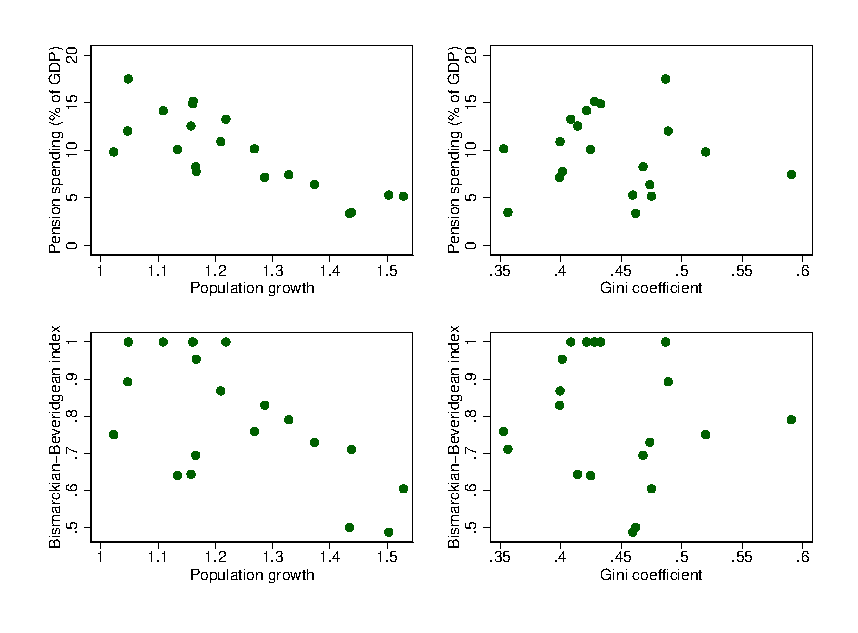
\includegraphics[width=\linewidth]{Figs/OECDdata.eps}
\end{figure}

The paper closest to ours is \textcite{CondeRuizP07a1}, which shows that in certain OECD countries, greater income inequality is linked to Beveridgean systems with lower benefits. It explains these findings using a three-income-group overlapping generations model, where two types of equilibria might arise. If inequality is high, a coalition between the rich and poor will choose a small Beveridgean system, whereas if inequality is low, the middle class will favor a Bismarckian system with a higher tax rate. XXX In contrast with this theory, data for twenty rich OECD countries in 2020 show no clear relation between pension spending, or the degree by which benefits are Bismarckian or Beveridgean, with income inequality; see figure \ref{fig:US:OECDdata}.\footnote{The countries are Australia, Austria, Belgium, Canada, Denmark, Finland, France, Germany, Iceland, Ireland, Italy, Japan, Netherlands, New Zealand, Norway, Spain, Sweden, Switzerland, United Kingdom, United States. Pension spending, population growth, and Bismarckian-Beveridgean index from OECD data, the later is the ratio of the replacement rates at mean income and half mean income, see section \ref{sec:quant}. Population growth is the ratio of population in 2020 and population in 1990 (there is no correction for differences in retirement age, see \ref{sec:quant}). Gini coefficient are from World Income Inequality Database. All data is for 2020} At the same time there is a clear pattern between these two variables and population growth. XXX Our model provides a rationale for the latter XXX. Furthermore, in our work, social security systems differ along two dimensions, and our model provides a quantitative evaluation of the impact of system characteristics on the tax rate, labor supply, and savings. 


The rest of the paper is organized as follows: Section \ref{sec:model} presents the economic environment and the economic and politico-economic equilibrium concepts. Section \ref{sec:LOG} considers GHH preferences with logarithmic utility and analyzes politico-economic equilibria under different pension systems. In section \ref{sec:quant}, we calibrate the model to Argentina to quantify the effects of a pension reform that expanded the system to universal coverage. We also calibrate the model to the United States, France, and the United Kingdom in order to identify the main determinants of equilibrium tax rates, labor supply, and capital accumulation. Section XXX considers the political choice of system characteristics and evaluates its determinants by looking at United States, France, and the United Kingdom. Section \ref{sec:conclu} concludes, and an appendix collects proofs, auxiliary calculation, discussion of numerical methods, and other ancillary discussions. 



